\documentclass{beamer}
\usepackage[utf8]{inputenc}
\usepackage[portuguese]{babel}
\usepackage{graphicx}
\usepackage[font=tiny]{caption}

\graphicspath{{./Imagens/}}

%\usetheme{Warsaw}
%\usetheme{Madrid}
%\usetheme{Antibes}
\usetheme{Berkeley}
%\usecolortheme{wolverine}

\title{V Workshop de taiko}
\author{Osasco Todorokidaiko}
\date{25 de Agosto de 2019}

\begin{document}
\begin{frame}
    \maketitle
\end{frame}

\section{História}
\subsection{Origem}
\begin{frame}{Origem do taiko}\pause
    Era Joumon

    Cerca de 2000 anos
    \begin{figure}
    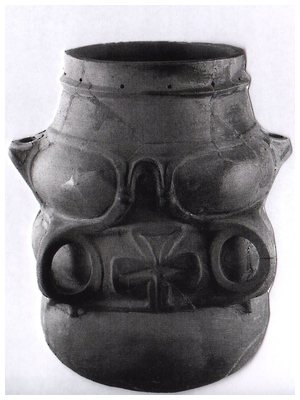
\includegraphics[height=2cm]{taiko-jomon}
        \caption {Tambor de argila escavado na prefeitura de Nagano.}
    \end{figure}

\end{frame}

\begin{frame}{Usos}
    \begin{itemize}\pause
        \item Comunicação \pause
        \item Religião \pause
        \item Festivais \pause
        \item Guerra
    \end{itemize}
\end{frame}

\subsection{Usos tradicionais}
\begin{frame}{Com o passar dos séculos...}
    \pause
    \begin{itemize}
        \item Gagaku

            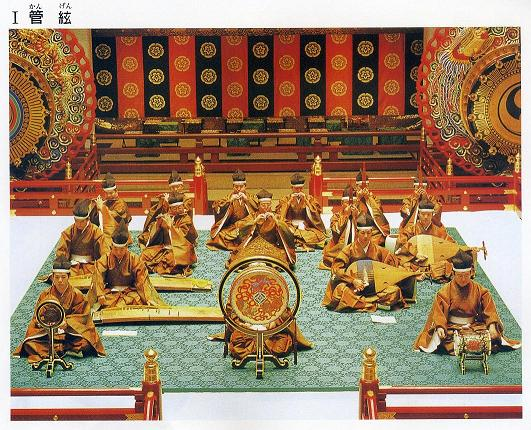
\includegraphics[height=1.7cm]{gagaku-1}
            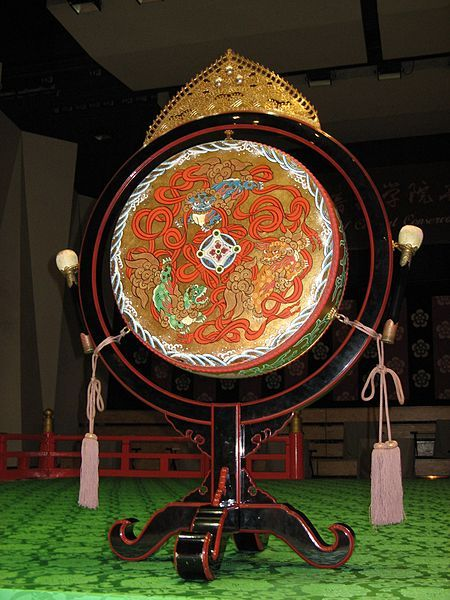
\includegraphics[height=1.7cm]{gagaku-2}
            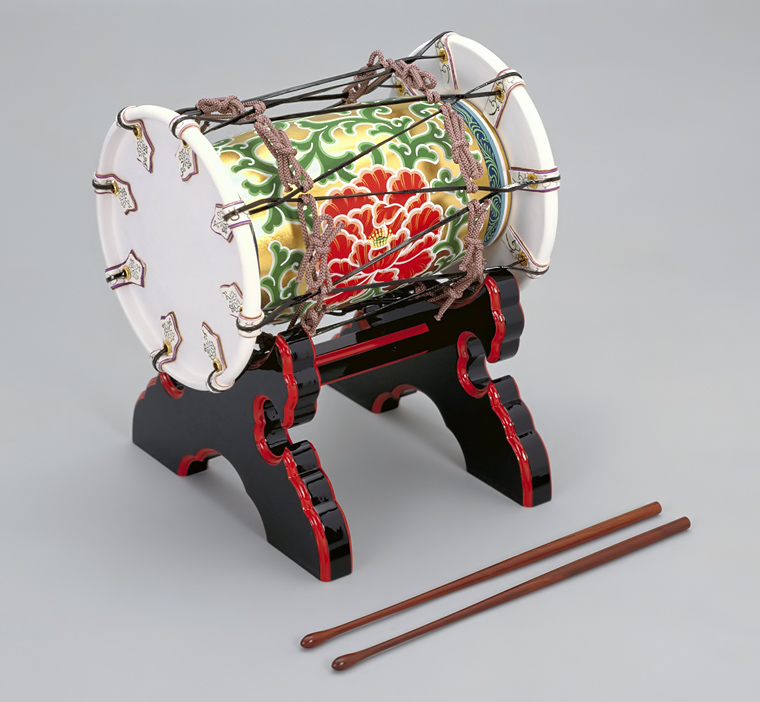
\includegraphics[height=1.7cm]{gagaku-3}
            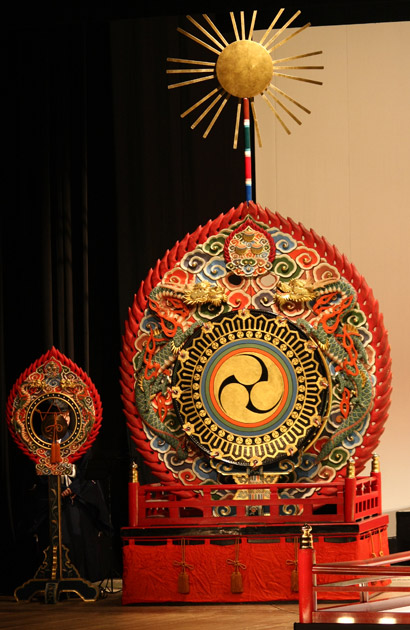
\includegraphics[height=1.7cm]{gagaku-4}
            \pause
        \item Kabuki

            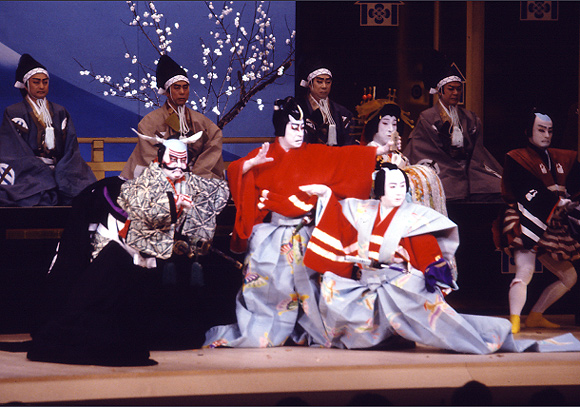
\includegraphics[height=1.7cm]{kabuki-1}
            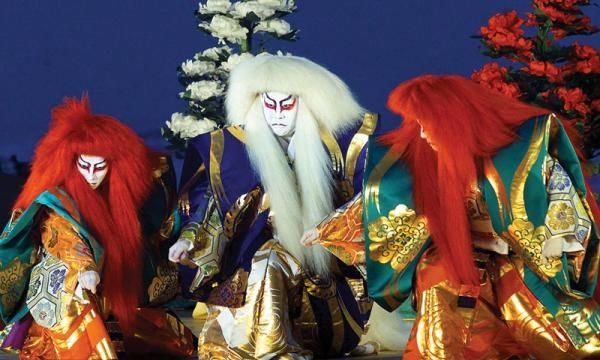
\includegraphics[height=1.7cm]{kabuki-2}
            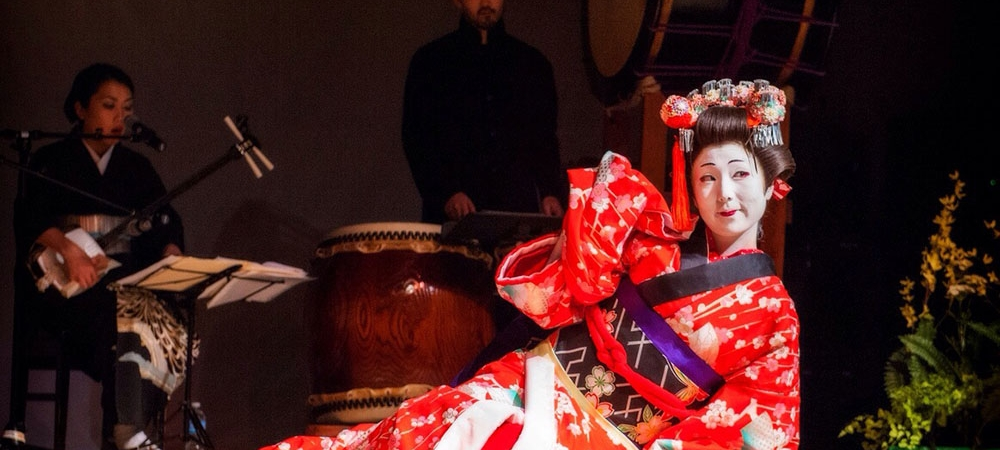
\includegraphics[height=1.7cm]{kabuki-3} 
            \pause
        \item Bon odori
            
            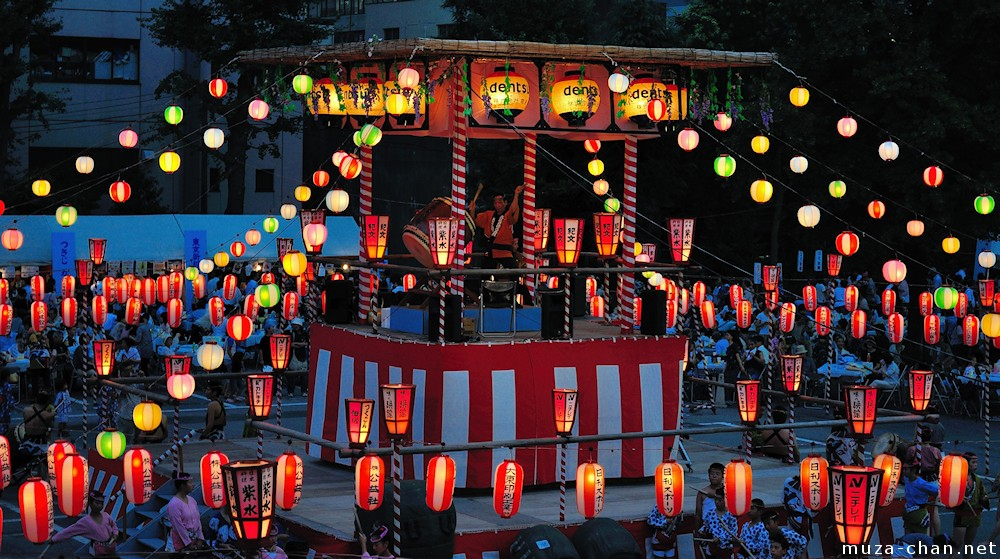
\includegraphics[height=1.7cm]{bonodori-1}
            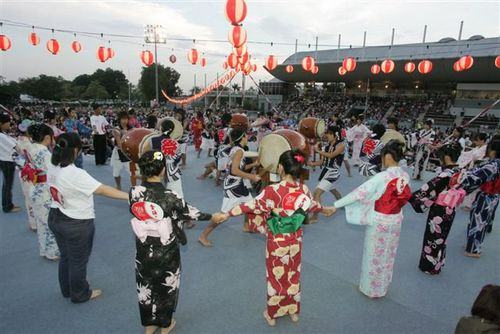
\includegraphics[height=1.7cm]{bonodori-2}
            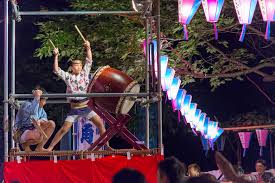
\includegraphics[height=1.7cm]{bonodori-3} 
            \pause
        \item Entre outros...
    \end{itemize}    
\end{frame}

\subsection{Taiko moderno}
\begin{frame}{Taiko moderno}
    \pause
    1951 - Daihachi Oguchi
    
    \textbf{Kumidaiko}: Várias pessoas tocando vários taikos diferentes
    \pause

    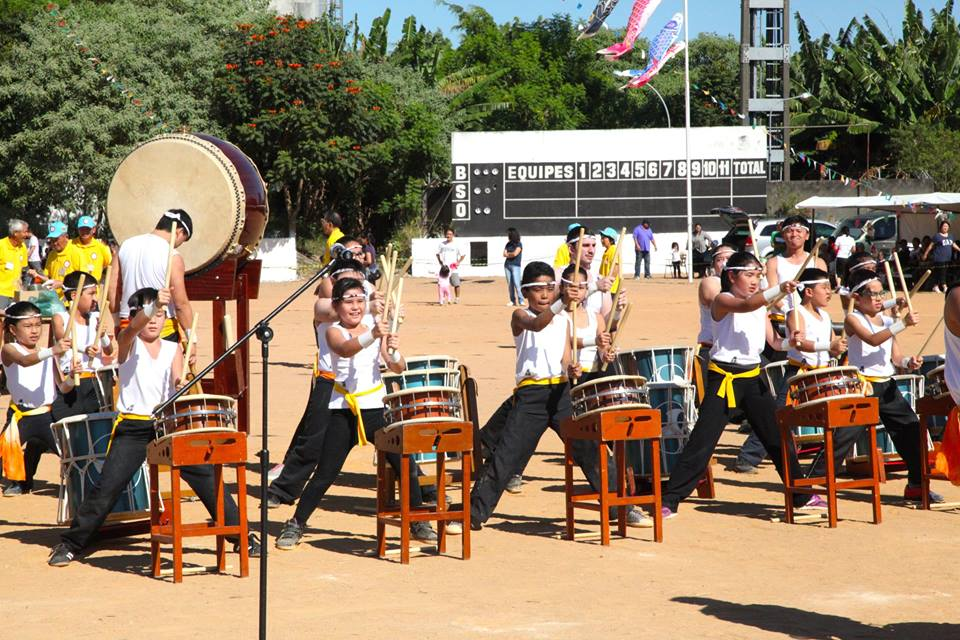
\includegraphics[height=3cm]{kumidaiko-1}
    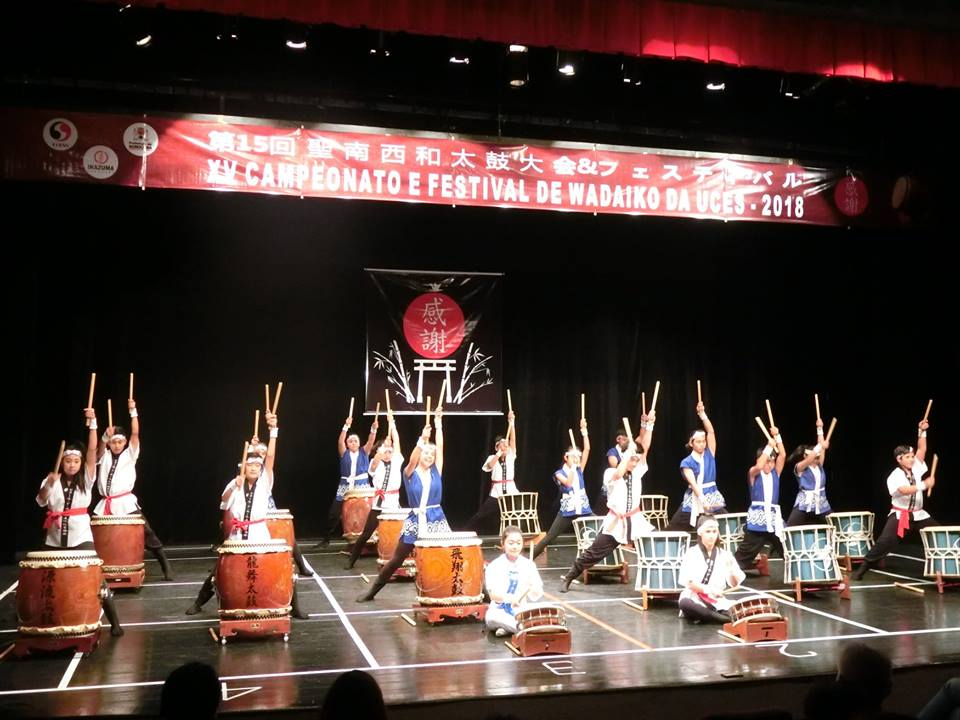
\includegraphics[height=3cm]{kumidaiko-2}
    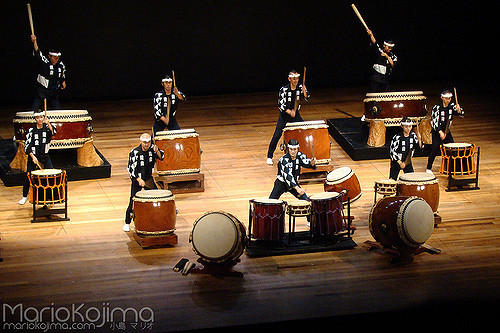
\includegraphics[height=3cm]{kumidaiko-3}
    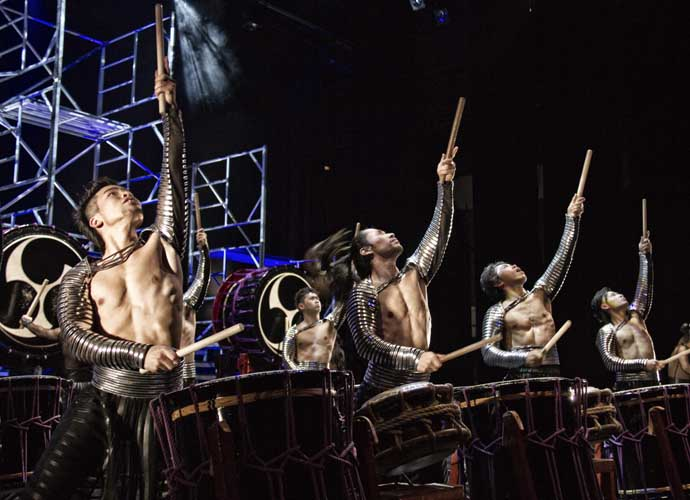
\includegraphics[height=3cm]{kumidaiko-4}
    
\end{frame}

\subsection {No Brasil}
\begin{frame}{No Brasil}
    \pause
    \begin{itemize}
        \item Imigrantes\pause
        \item 2002: Associação Fukuoka do Brasil\pause

            6 taikos doados de Fukuoka e a vinda do sensei Yokihisa Oda.
            \begin{figure}
                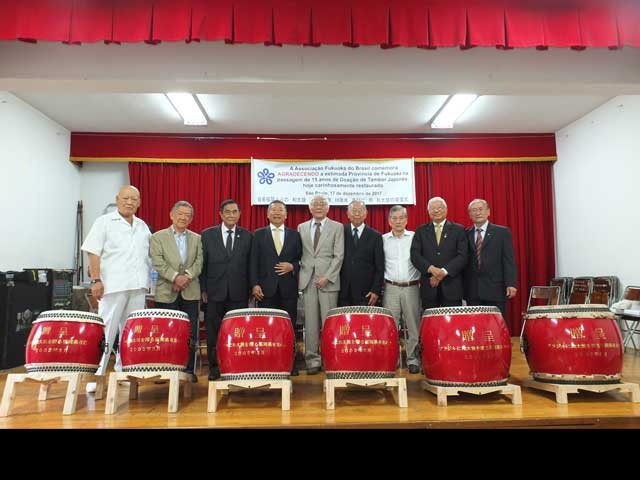
\includegraphics[height=2cm]{fukuoka}
            \end{figure}
    \end{itemize}\pause
    Desde então vários grupos foram formados e o instrumento se popularizou em muitas regiões do Brasil
\end{frame}

\begin{frame}{No Brasil}
    Atualmente...\pause
    \begin{itemize}
        \item Associação Brasileira de Taiko (ABT)
            \pause
        \item Campeonatos e festivais brasileiros
            \pause
        \item Regionais
            \pause
        \item Mais de 60 grupos associados e cerca de 150 reconhecidos.
    \end{itemize}
\end{frame}

\subsection {Nosso grupo}
\begin{frame}{Nosso grupo}
    \pause
    \begin{itemize}
        \item Fundado em 2003
            \pause

        \item Campeão brasileiro da categoria Júnior em 2010 e da categoria Mirim em 2017 e campeão da sudoeste nos anos de  2008, 2011 e 2012.
            \pause

        \item Atualmente com cerca de 25 tocadores
    \end{itemize}
\end{frame}

\begin{frame}{Undokai}
    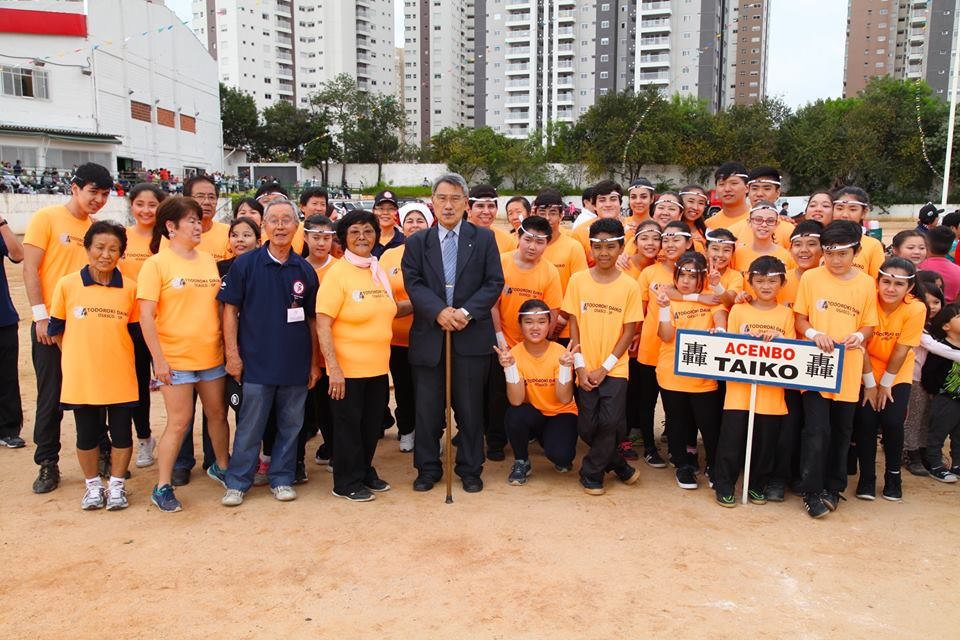
\includegraphics[height=3cm]{undokai-1}
    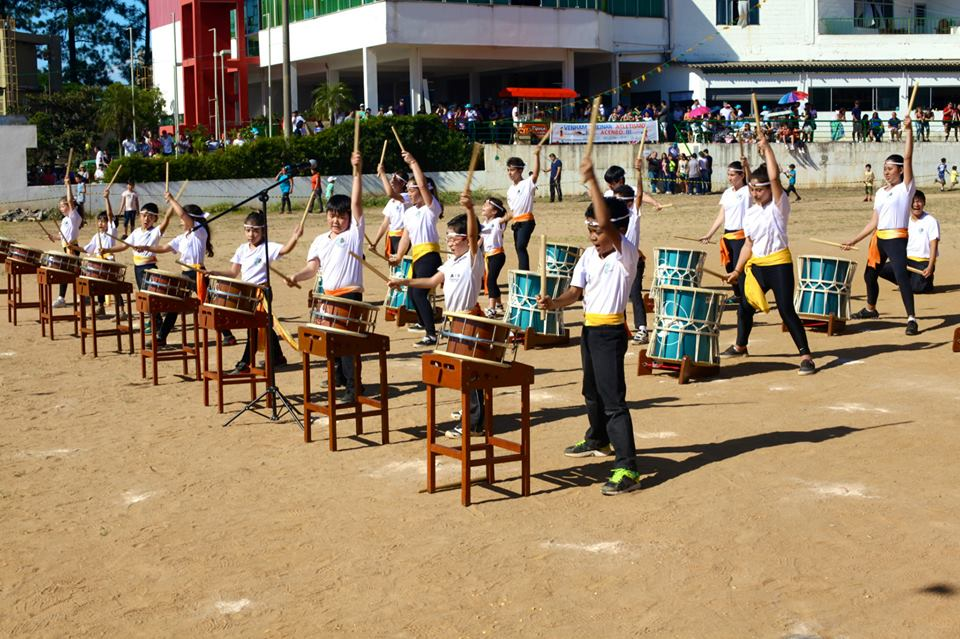
\includegraphics[height=3cm]{undokai-2}
    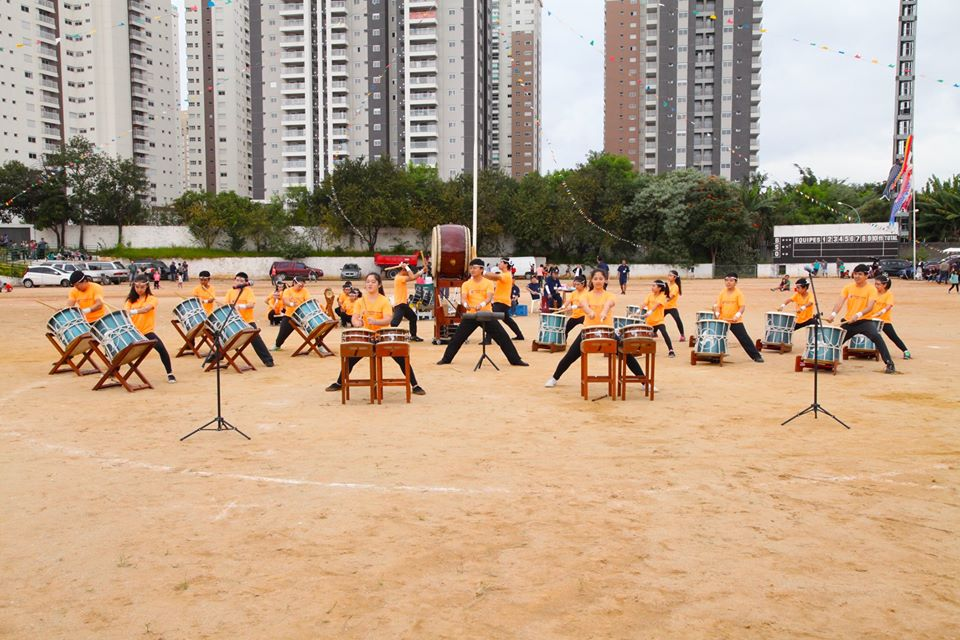
\includegraphics[height=3cm]{undokai-3}
    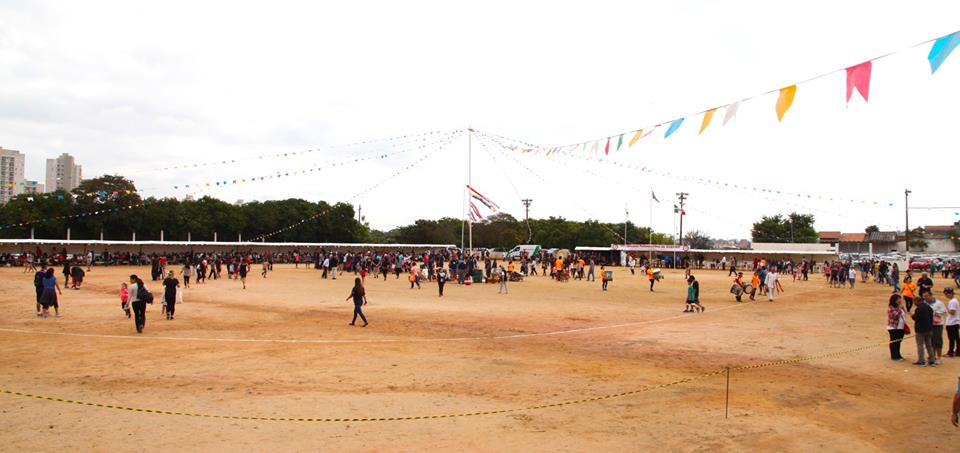
\includegraphics[height=2cm]{undokai-4}
\end{frame}

\begin{frame}{Ikoi no Sono}
    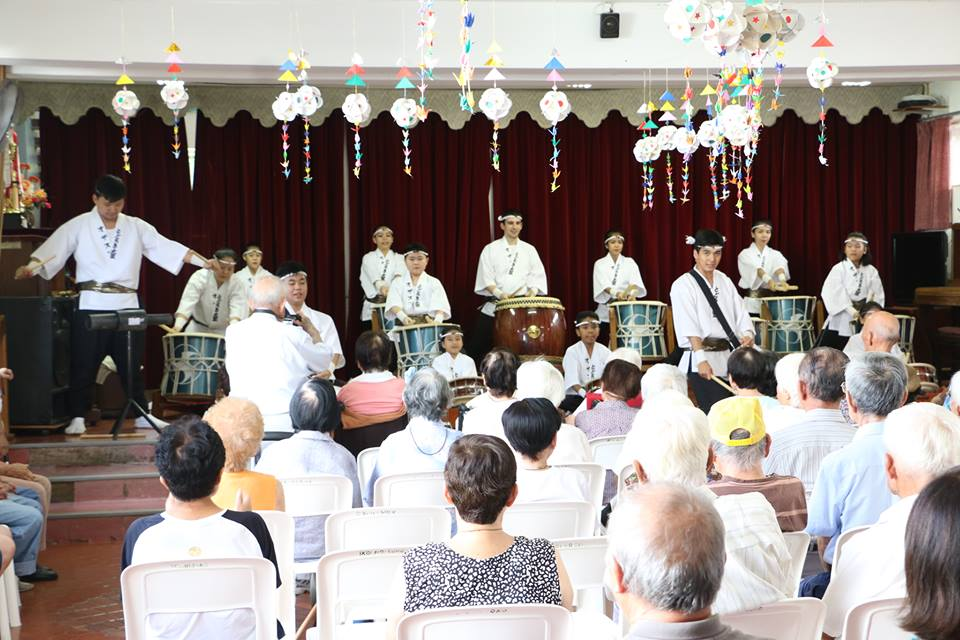
\includegraphics[height=3cm]{ikoi-no-sono-1}
    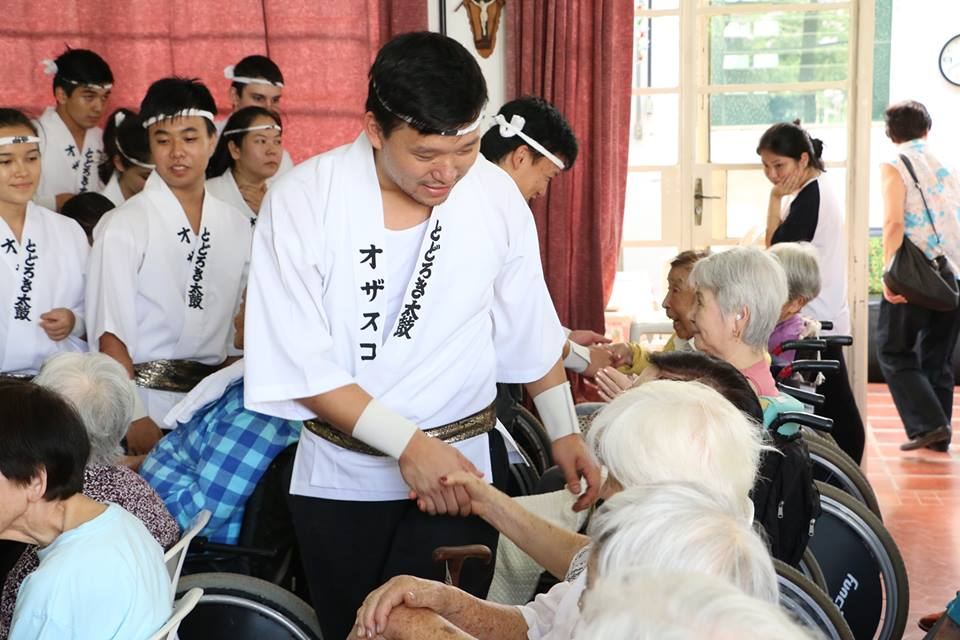
\includegraphics[height=3cm]{ikoi-no-sono-2}
    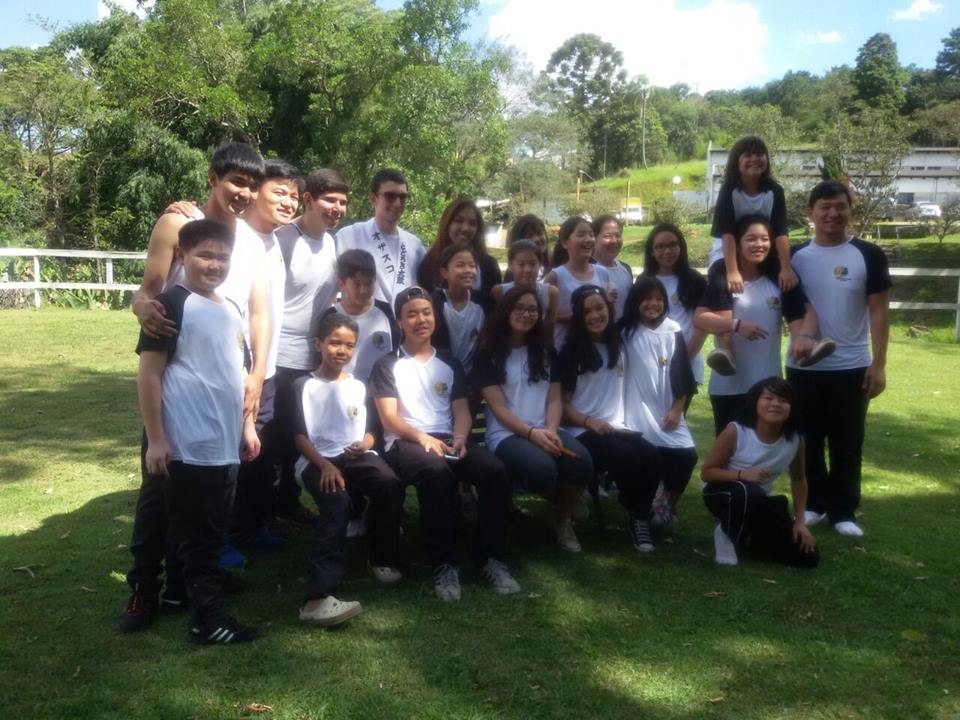
\includegraphics[height=3cm]{ikoi-no-sono-3}
    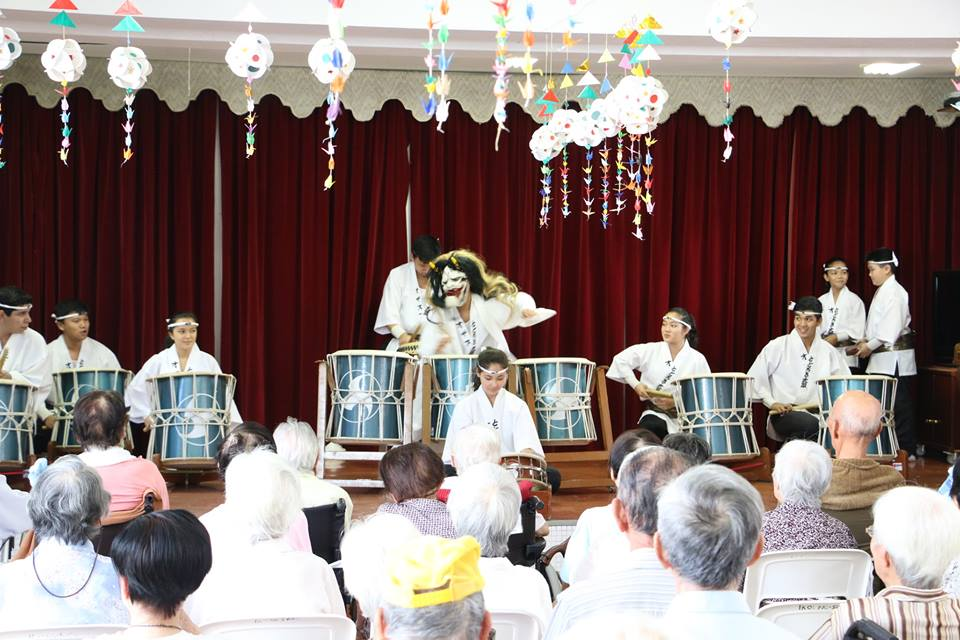
\includegraphics[height=3cm]{ikoi-no-sono-4}
\end{frame}

\begin{frame}{Japan Matsuri}
    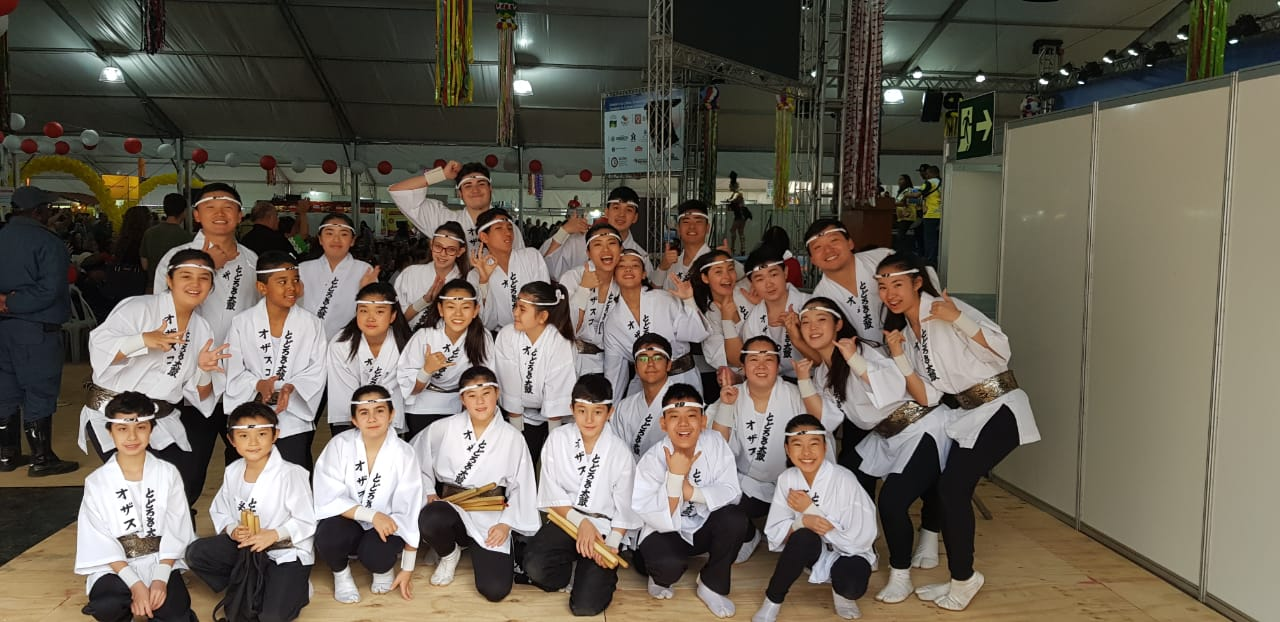
\includegraphics[height=3cm]{JM-1}
    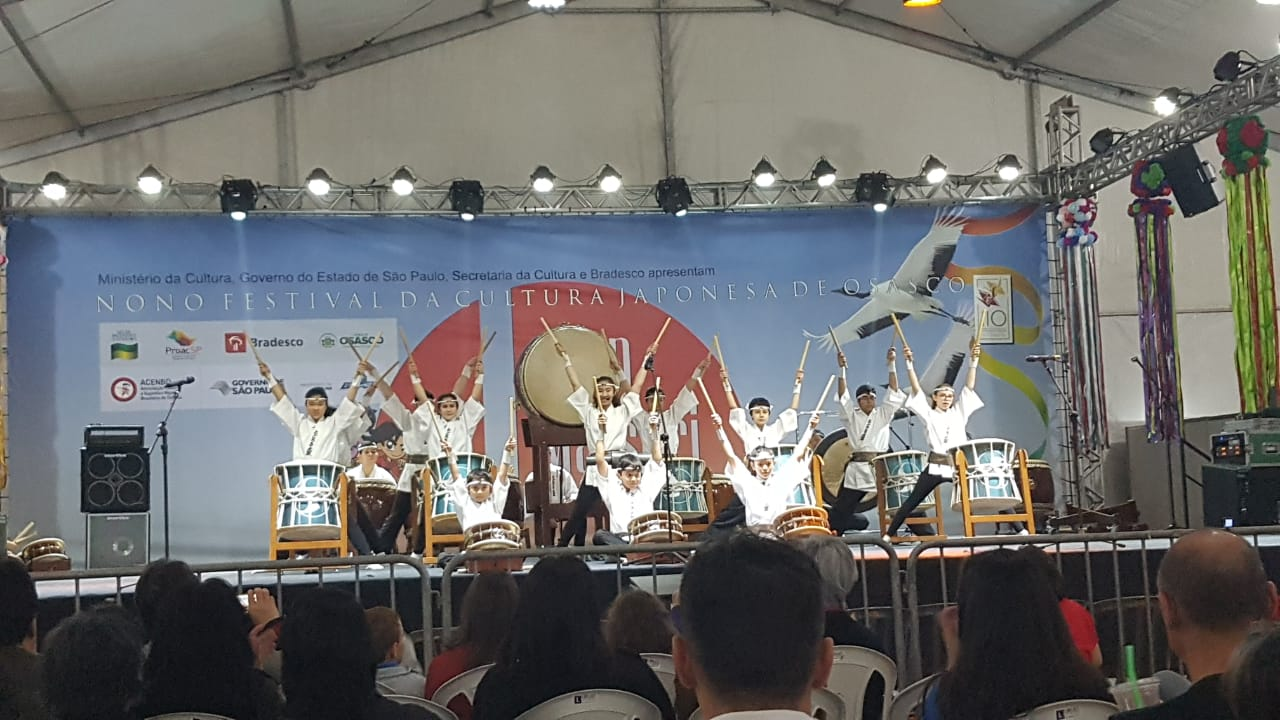
\includegraphics[height=3cm]{JM-2}
\end{frame}

\begin{frame}{Campos do Jordão}
    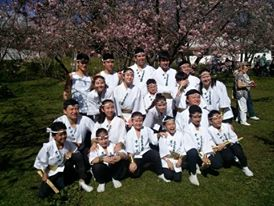
\includegraphics[height=3cm]{campos-1}
    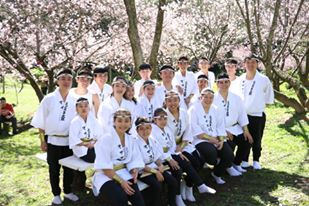
\includegraphics[height=3cm]{campos-2}
\end{frame}

\begin{frame}{Todoroki Fest}
    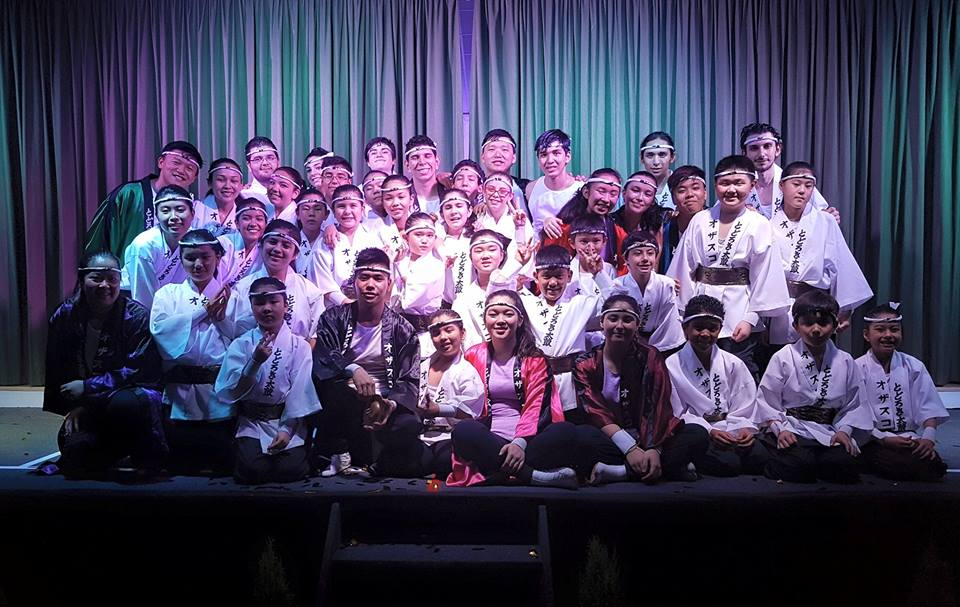
\includegraphics[height=3.1cm]{todoroki-fest-1}
    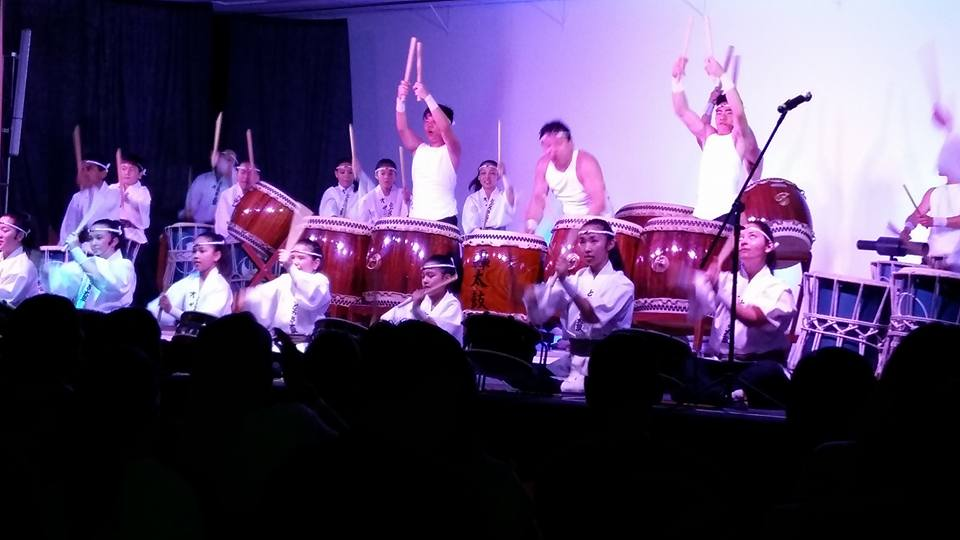
\includegraphics[height=3.1cm]{todoroki-fest-2}
\end{frame}



\section {Curiosidades}
\subsection {Instrumentos}
\begin{frame}{Instrumentos}
    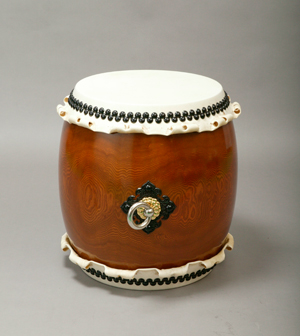
\includegraphics[height=0.2\textheight]{instrumentos-1}
    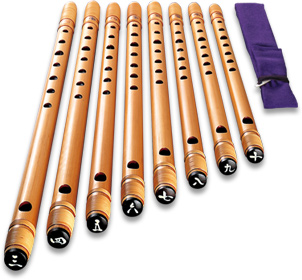
\includegraphics[height=0.2\textheight]{instrumentos-2}
    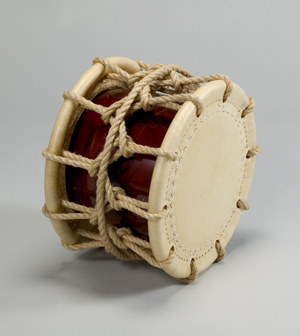
\includegraphics[height=0.2\textheight]{instrumentos-3}
    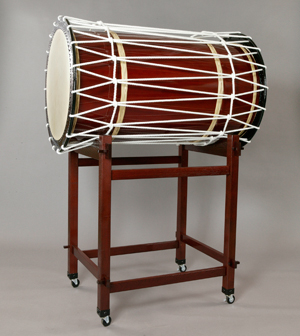
\includegraphics[height=0.2\textheight]{instrumentos-4}
    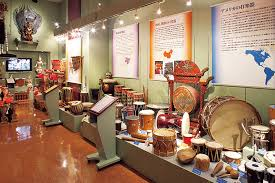
\includegraphics[height=0.2\textheight]{instrumentos-5}
    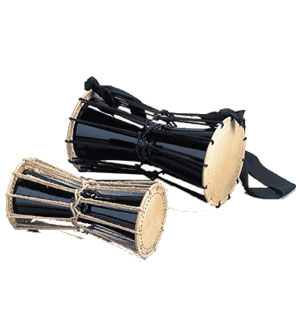
\includegraphics[height=0.2\textheight]{instrumentos-6}
    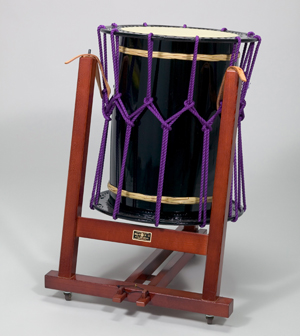
\includegraphics[height=0.2\textheight]{instrumentos-7}
    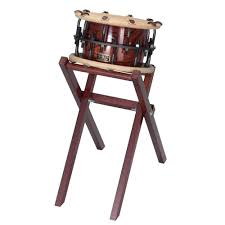
\includegraphics[height=0.2\textheight]{instrumentos-8}
    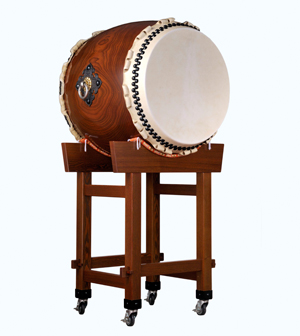
\includegraphics[height=0.2\textheight]{instrumentos-9}
    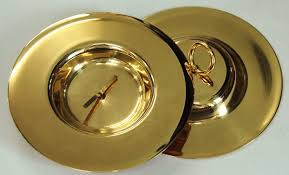
\includegraphics[height=0.2\textheight]{instrumentos-10}
    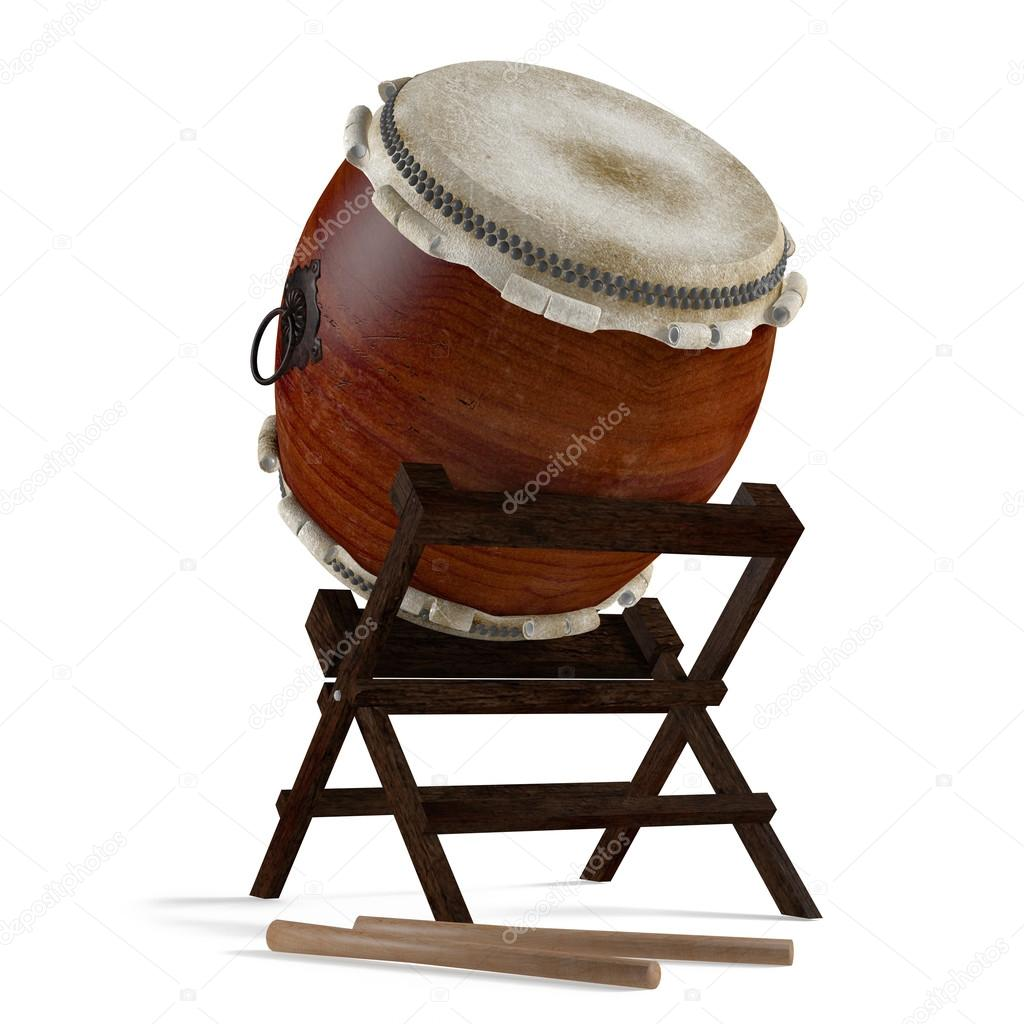
\includegraphics[height=0.2\textheight]{instrumentos-11}
    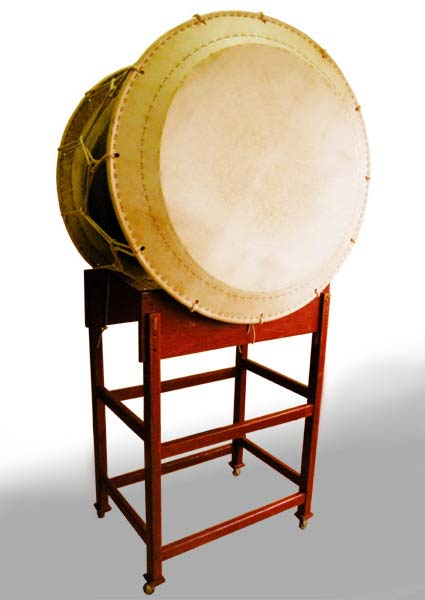
\includegraphics[height=0.2\textheight]{instrumentos-12}
    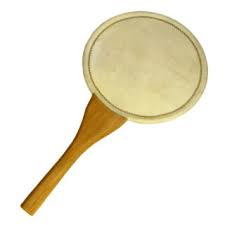
\includegraphics[height=0.2\textheight]{instrumentos-13}
    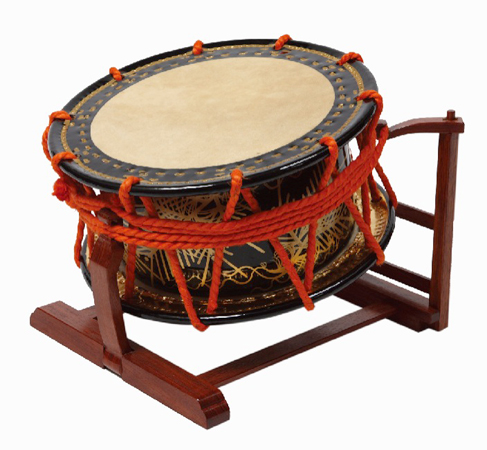
\includegraphics[height=0.2\textheight]{instrumentos-14}
    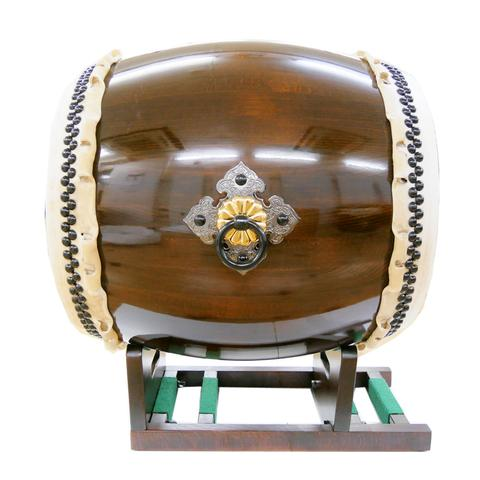
\includegraphics[height=0.2\textheight]{instrumentos-15}
\end{frame}

\subsection {Entreterimento}
\begin{frame}{Entreterimento}
    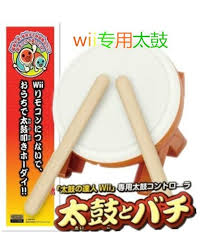
\includegraphics[height=0.4\textheight]{wii}
    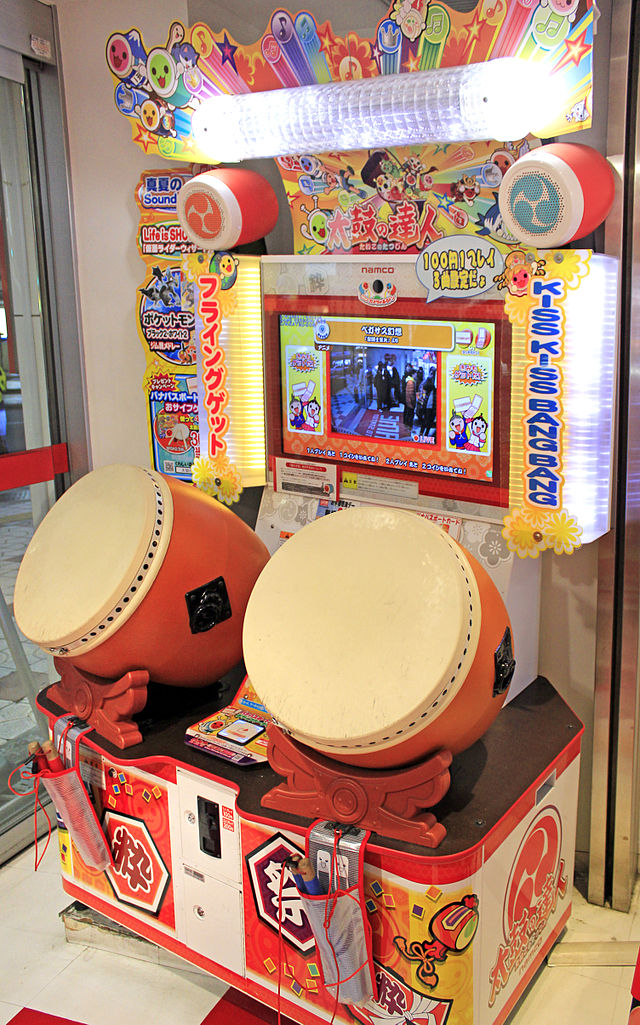
\includegraphics[height=0.4\textheight]{tatsujin}
    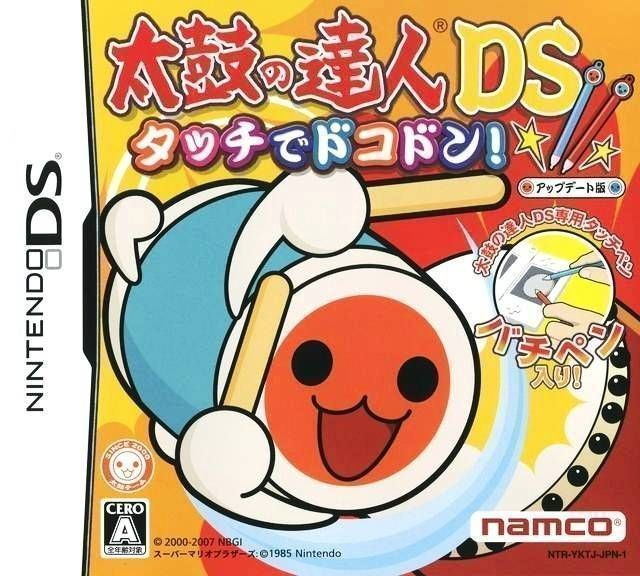
\includegraphics[height=0.4\textheight]{ds}
\end{frame}
\end{document}
